\hypertarget{2}{}

\rhead{Biomedical Relation Extraction}
\lhead{Chapter 2}

\chapter[Biomedical Relation Extraction]
{\huge Biomedical Relation Extraction}

\vspace{-1.6cm}

% Gray Line
\begingroup
\color{black}
\par\noindent\rule{\textwidth}{0.4pt}
\endgroup

\noindent{This chapter provides an overview of the key concepts to understand biomedical Relation Extraction (RE) according to the two main objectives established in Chapter \hyperlink{1}{1}. It also presents some of the approaches for RE by order of complexity and the methods/steps needed for their evaluation. The chapter corresponds to a combination of two review articles as mentioned in the introductory chapter: \hyperlink{AA}{Appendix A} \citep{sousa2021using} and \hyperlink{AB}{Appendix B}.}

\section{Learning for Relation Extraction}

Using different sources of information to support the automated extraction of relations between biomedical concepts contributes to the development of our understanding of biological systems. Researchers have proposed several RE approaches to identify relations between concepts in biomedical literature, namely, using neural network algorithms. The possibility of using multichannel architectures composed of multiple data representations, as in deep neural networks, leads to state-of-the-art results. The right combination of data representations can eventually lead us to even higher evaluation scores in RE tasks. The following sections will present the baseline concepts that are the building blocks for RE, the initial approaches to performing RE, and the different approaches, systems, and evaluation practices for deep learning RE.  

\hypertarget{2.1.1}{\subsection{Natural Language Processing}}

Natural Language Processing (NLP) is a field in computer science that aspires to obtain meaning from highly heterogeneous or unstructured text written by humans. This field covers several techniques that constitute pre-processing steps for the tasks described in the following section. NLP techniques target different goals and are often combined to obtain higher performance:

\begin{itemize}
    \item \textbf{Tokenization} breaks the text into tokens to be processed individually or as a sequence. The tokens are usually words but can also be phrases, numbers, and other types of elements. The most straightforward form of tokenization is breaking the input text by whitespaces or punctuation. However, with literature that is descriptive and formal, we have to account for complex entities. These entities tend to be morphologically complex and need specialized tokenization pipelines. Some researchers use a compression algorithm \citep{sennrich2015neural}, byte pair encoding (BPE), to account for vocabulary variability. BPE represents open vocabularies through a fixed-size vocabulary of variable-length character sequences, making it suitable for neural network models, for instance.

    \item \textbf{Stemming and Lemmatization} reduces the variability of natural language by normalizing a token to its base form (stem) \citep{manning2008introduction}. Also, it can take into account the context of the token, along with vocabulary and morphological analysis, to establish the canonical form of the word (lemma). The lemma is always a real word, but the stem can correspond only to a fragment of a word. For example, the stem of the word \textit{having} is \textit{hav}, and the lemma is \textit{have}.

    \item \textbf{Part-of-Speech (POS) Tagging} assigns each word of a sentence to the category where it belongs, taking into account its context (e.g., adverb or preposition). Each word can belong to one or more categories. This feature expresses the role of a word in a given sentence. 

    \item \textbf{Parse Tree} represents the syntactic structure of a sentence. There are two types of parse trees: constituency-based parse trees and dependency-based parse trees. The main difference between the two is the distinction between the terminal and non-terminal nodes. The first makes that distinction, and in the second, all nodes are terminal. In constituency-based parse trees, each node of the tree is either a \textit{branch} node, a \textit{leaf} node, or a \textit{root} node. For each sentence, there is only one \textit{root} node. The \textit{leaf} node is terminal, and the \textit{branch} node connects to two or more \textit{child} nodes. These leaves correspond to the lexical tokens \citep{aho1986compilers}. Dependency-based parse trees are usually simpler because they only identify the primary syntactic structure, leading to fewer nodes. The structures created by parse trees are used as inputs for other algorithms and can be constructed based on supervised learning techniques.
\end{itemize}

\hypertarget{2.1.2}{\subsection{Text Mining Primary Tasks}}

Text mining is a widespread approach to identifying and extracting information from unstructured or highly heterogeneous text \citep{westergaard2018comprehensive}. Text mining is used to extract facts and relationships in a structured form that can be used to annotate specialized databases and transfer knowledge between domains \citep{fleuren2015application}. Text mining can be considered as a sub-field of data mining. Thus, with the transformation of text into appropriate data representations, we can apply data mining algorithms, namely numeric vectors. In recent years, text mining tools have evolved remarkably in quality and number, but there are still several challenges in applying text mining to scientific literature. The main challenges are the heterogeneity and complexity of the written resources, making the retrieval of relevant information (i.e., relations between entities) a non-trivial task. 

Text Mining tools can target different tasks separately or together. Some primary tasks are detailed below, including RE. 

\begin{itemize}
    \item \textbf{Topic Modelling:} the classification of documents according to their topics or themes. This task aims to organize a set of documents to identify which documents are more relevant to a given topic \citep{blei2012probabilistic}. Related tasks include document triage \citep{buchanan2007investigating} and document clustering.

    \item \textbf{Named Entity Recognition (NER):} consists of identifying entities that are mentioned in the text. In most cases, the exact location of each entity in the text is required, given by the offset (position) of its first and last characters. In some cases, discontinuous entities may be considered, requiring multiple offset pairs. The classification of entity properties such as its type (e.g., protein, cell line, chemical) can be included in this task \citep{nadeau2007survey}.

    \item \textbf{Normalization:} consists of matching each entity to an identifier belonging to a knowledge base that unequivocally represents its  concept. For example, a protein may be mentioned by its full name or an acronym; in this case, the normalization process should assign the same identifier to both occurrences. The identifiers can be provided by an external database or ontology \citep{tsuruoka2008normalizing}. Similar tasks include named entity disambiguation \citep{bunescu2006using}, named entity linking (NEL), and harmonization.

    \item \textbf{Relation Extraction (RE):} the identification of entities that participate in a relationship described in the text. Most tools consider relations between two entities in the same sentence, but some focus on $n$-ary relations (between more than two entities) across multiple sentences \citep{singhal2016text}. Biomedical relations commonly extracted are gene-phenotype and drug-drug interactions \citep{segura2014lessons}.

    \item \textbf{Event Extraction:} can be considered an extension of the RE task, where the label of the relation and role of each participant is specified. The events extracted should represent the mechanisms described in the text \citep{Ananiadou2010}. Related tasks include slot-filling and relation classification.

    \item \textbf{Question Answering (QA):} is a task where we aim to automatically answer questions asked by humans in natural language using either an existing structured database or a collection of natural language documents \citep{CALIJORNESOARES2020635}.
\end{itemize}

\subsection{Initial Approaches}

Through the years, RE approaches became increasingly more intricate with the associated growth in performance. This section describes the RE approaches and some of their applications that preceded the deep learning-based RE systems. Due to the inherent complexity of highly heterogeneous or unstructured literature, initial approaches for RE worked on a sentence level \citep{lamurias2017extracting} and focused primarily on binary relations \citep{zhang2017review}.

\subsubsection{Co-occurrence}

Co-occurrence assumes that if two entities are mentioned in the same sentence (co-occur), they are likely related. Usually, this approach's application results in a higher recall (most entities co-occurring in a sentence participate in a relation) and lower precision. 
Some methods use frequency-based scoring schemes to eliminate relations identified by chance \citep{zweigenbaum2007frontiers}. Nowadays, applications occasionally use co-occurrence as a baseline against more complex approaches \citep{bunescu2006integrating}. 

\hypertarget{2.1.3.2}{\subsubsection{Pattern-based}}

Pattern-based uses manually defined patterns and automatically generated patterns to extract relations.

\textbf{Manually defined patterns} require domain expertise knowledge about the type of entities, their interactions, and the subject. 
Initial systems made use of regular expressions to match word patterns that reflected a relation between two entities \citep{smolinski2009computational}, making use of a dictionary of words that express relation, such as \textit{trigger} and \textit{stimulate}. Later systems introduce POS tagging, but this has proven to be too naive, mainly when applied to complex sentences, such as the ones that we typically find in scientific literature \citep{hao2005discovering}. Opposite to the co-occurrence approaches, manually defined patterns frequently achieve high precision but tend to have a poor recall. This approach does not generalize well and therefore is difficult to apply to new unseen data. 

\textbf{Automatically generated patterns} encompass two main approaches, bootstrapping with seeds \citep{wang2011inference} and leveraging of the corpora \citep{liu2011graphs}. 
The bootstrapping method uses a small set of relations known as seeds (e.g., person-occupation pairs). The first step is to identify the seeds in the dataset and map the relation pattern they describe. The second step is to try to apply the mapped patterns to the dataset to identify new pairs of relations that follow the same construction. Finally, the original set of relations is expanded by adding these new pairs. When, after repeating all previous steps, no more pairs are found, the process ends. Some systems apply distant supervision techniques to keep track of the validity of the added patterns. Distant supervision uses existing knowledge base entries as gold standards to confirm or discard a relation \citep{jiang2018revisiting}. This method is susceptible to noisy patterns as the original set of relations grows.
On the other hand, the leveraging of the corpora method makes immediate use of the entire dataset to generate the patterns. This method requires a higher number of annotated relations and produces highly specific patterns that cannot match new unseen data. Automatically generated patterns can achieve higher recall than manually defined patterns, but overall the noisy patterns continue to damage the precision. Nevertheless, there were a few efforts to reduce the number of noisy patterns \citep{nguyen2010simple}. 

\subsubsection{Rule-based}

Rule-based also uses manually defined and automatically generated rules from the training data to extract relations. Depending on the systems, the differences between pattern-based and rule-based approaches can be minor. 
Ruled-based approaches use not only patterns but also additional restraints to cover issues that are difficult to express by patterns, such as checking for the negation of the relations \citep{koike2005automatic}. Some ruled-based systems distance themselves from pattern-based approaches by replacing regular expressions with heuristic algorithms and sets of procedures \citep{rinaldi2007mining}. Like pattern-based approaches, ruled-based approaches tend to have a poor recall, even though rules tend to be more flexible. The trade-off recall/precision can be improved using automatic methods for rule creation \citep{xu2012feature}.

\subsubsection{Machine Learning (ML)}

Accordingly to the types of corpora, researchers divide RE based on machine learning into three domains \citep{zhang2017review}: supervised learning methods, semi-supervised learning methods, and unsupervised learning methods, beyond the deep learning methods described in Section \hyperlink{2.1.4}{2.1.4}. 

\textbf{Supervised machine learning} uses large annotated corpora to perform RE. These corpora are pre-processed using NLP tools and then used to train classification models. It is possible to categorize these ML methods into two main approaches, Feature-based and Kernel-based. \textbf{Feature-based approaches} represent each instance (e.g., a sentence) as a vector in an $n$-dimensional space. Support Vector Machines (SVM) classifiers tend to be used to solve binary classification problems and are considered black boxes because it can be difficult to interpret and understand the underlying decision-making process. These classifiers can use different features that are meant to represent the data characteristics (e.g., shortest path, bag-of-words (BOW), and POS tagging) \citep{kim2008detection}. \textbf{Kernel-based approaches} main idea is to quantify the similarity between the different instances in a dataset by computing the similarities of their representations \citep{giuliano2006exploiting}. Kernel-based approaches add the structural representation of instances (e.g., by using parse trees). These methods can use one kernel or a combination of kernels (e.g., graph, sub-tree (ST), and shallow linguistic (SL)). SVM classifiers do not need to use kernels. However, kernels are commonly used in these classifiers to the point where their use is subtended by most users. 

\textbf{Semi-supervised or weekly supervised learning} methods mainly encompass the bootstrap method described previously (Section \hyperlink{2.1.3.2}{2.1.3.2}) \citep{hoffmann2011knowledge,augenstein2015extracting}. It is mostly used in the field of knowledge extraction to solve classification and RE problems. 
This learning method reduces the dependence on human participation and corpus annotation. However, the bootstrap method has the problem of semantic drift when in the iterative process, damaging the RE's performance.

Supervised and semi-supervised learning methods need to determine the type of relation in advance. Large-scale corpora implies multiple relations, and most of the time, those methods are not able to grasp all of that variety. 

\textbf{Unsupervised learning} was first used to grasp a more varied pool of relations based on clustering \citep{hasegawa2004discovering,shinyama2006preemptive}. 
The idea was to use text information clustering between two entities to express the relation class. This formulation was successfully applied to multiple approaches and improved to multilevel clustering by \cite{shinyama2006preemptive}. In unsupervised learning, some researchers also developed methods based on pattern clustering (i.e., Density-based methods) and sentence parsing \citep{quan2014unsupervised}. 
This category of methods makes it hard to describe the relation name accurately and has difficulties catching low-frequency relations (i.e., leading to low recall).


\hypertarget{2.1.4}{\subsection{Deep Learning}}

Artificial neural networks are a parallel combination of small processing units (nodes) which can acquire knowledge from the environment through a learning process and store the knowledge in the connections between the nodes \citep{haykin1994neural} (represented by direct graphs \citep{guresen2011definition}). The process is inspired by the biological brain function, having each node corresponding to a \textit{neuron} and the connections between the nodes representing the \textit{synapses}. Artificial neural networks use fully connected layers to connect every neuron in one layer to every neuron in another layer. 
The first application of neural networks to NLP was language modelling, which has been useful in learning distributed representations (embeddings) for words \citep{bengio2003neural,mikolov2013distributed}. These data representations (i.e., word embeddings) were the initial step for a new way to successfully perform several NLP tasks based on neural networks \citep{nguyen2015relation}.  


\subsubsection{Convolutional Neural Networks (CNN)}

Some deep learning RE systems use Convolutional Neural Networks (CNN) to further encode the sentences, capturing $n$-gram level features. CNN consists of three parts: the input layer; the output layer; and several hidden layers, including convolutional layers, pooling layers, fully connected layers, and normalization layers \citep{xue2018relation}. 
In the convolutional layers, a convolution operation reduces the number of free parameters in the following way. Given an input sentence $x$ as a sequence of vectors $x = \{w_1,w_2,...,w_m\},\ w_i \in \mathbb{R}^d$, where $w_i$ represents the words in the $x$ sentence,  $m$ is the size of the input sentence, and $d$ is the dimensionality of the embedding space. If we have $l$ as the window size for the convolutional layer kernel, then the vector for the $i$-th window is formed by concatenating the input vectors for that window:

\begin{equation}
    q_i = w_{i:i+l-1};\ (1 \leq i \leq m-l+1);\ q_i \in \mathbb{R}^{(d \times l)}
\end{equation}

Then, a single convolutional kernel could be represented by a weight vector $W$ and a bias $b$, and the output for the $i$-th window computed as:

\begin{equation}
    p_i= f (W'q_i+b)
\end{equation}

where $f$ is the activation function. The shape of the output of the convolutional kernel $p$ would be $p \in \mathbb{R} ^{(m-l+1)}$. If the convolutional layer was a set of $d_c$ convolutional kernels, the output of the layer would be of the shape $\mathbb{R} ^{d_c \times (m-l+1)}$.
The convolutional operation allows the network to be more in-depth with fewer parameters, passing the result to the pooling layers. These layers (and also convolutional layers) provide a fixed-size output matrix and reduce the output dimensionality while keeping the essential information. 

\hypertarget{2.1.4.2}{\subsubsection{Recurrent Neural Networks (RNN)}}

Recurrent Neural Networks (RNN) are artificial neural networks where the nodes' connections follow a contrary path to the data flux. Thus, RNNs can use their internal state, or \textit{memory}, to process each input sequence. 
%RNNs, like some deep learning techniques, aim to train classification models based on word embeddings, POS tagging, and other features. 
RNN classifiers have multilayer architectures, where each layer learns a different representation of the input data. This characteristic makes RNN classifiers flexible to multiple text mining tasks without requiring task-specific feature engineering. Hence, while training, RNN keeps remembering the context, and each state can be defined by:

\begin{equation}
    h_t = f(h_{t-1}, x_t)
\end{equation}

where $x_t$ refers to the input and $h_t$ symbolizes the output, at a given time ($t$). Then, to each state we apply an activation function:

\begin{equation}
    h_t = tanh(W_{hh} \times h_{t-1} + W_{hx} \times x_t)
\end{equation}

where $W$ is the weight, $h$ is the single hidden vector, $W_{hh}$ is the weight at the previous hidden state, $W_{hx}$ is the weight at the current input state, and $tanh$ is an activation function that implements a non-linearity that squashes the activations to the range $[-1,1]$. Then, the output state is:

\begin{equation}
    y_t = W_{hy} \times h_{t}
\end{equation}

where $W_{hy}$ is the weight at the output state.

\paragraph{Long Short-Term Memory Networks (LSTMs)}

Long Short-Term Memory (LSTM) networks are an alternative to regular RNN \citep{hochreiter1997long}. LSTMs are a type of RNN that handles long dependencies (e.g., sentences), making this classifier more suitable for scientific domains, for instance, where sentences are usually long and descriptive. LSTMs solve the vanishing problem of RNN using back-propagation, and its main constituents are three gates (the input gate, the output gate, and the forget gate).
In recent years, using LSTMs to perform RE tasks became widespread in various domains, such as semantic relations between nominals \citep{miwa2016end}. \textbf{Bidirectional LSTMs} use two LSTM layers at each step, one that reads the sentence from right to left, and other that reads from left to right. The combined output of both layers produces a final score for each step. Bidirectional LSTMs have yielded better results than traditional LSTMs when applied to the same datasets \citep{zhang2015bidirectional}.

\subsubsection{Transformers}

Transformers were first introduced in 2017 \citep{vaswani2017attention}, greatly improving the performance of many NLP tasks, including RE. Transformers' performance is based on their ability to capture long-range dependencies and process sequential data, such as sentences or time-series data, with a robust attention mechanism. The transformer architecture is based on two components: the encoder and the decoder. The encoder takes an input sequence and processes it in parallel to create a sequence of hidden representations, capturing the contextual information of each input token. The decoder, on the other hand, takes the encoder's output and generates an output sequence autoregressively, one token at a time, attending to the encoder's representations. BERT \citep{devlin2019bert}, GPT \citep{radford2018improving}, and T5 \citep{raffel2020exploring} are transformers-based systems that nowadays have become the foundation systems for most NLP approaches.

\hypertarget{2.1.4.4}{\subsubsection{Data Representations}}

The combination of multiple and different languages and entity-related data representations is vital for the success of neural network models dedicated to RE tasks. Some of these features were already described in Section \hyperlink{2.1.1}{2.1.1}, such as POS tagging and parse trees:

\begin{itemize}
    \item \textbf{Shortest Dependency Path} (SDP) is a feature that identifies the words between two entities mentioned in the text, concentrating the most relevant information while decreasing noise \citep{xu2015classifying}. 
    \item \textbf{WordNet Hypernyms} are a feature that helps to hierarchize entities, structuring words similar to direct acyclic graphs \citep{miller1998wordnet}. For example, a \textit{vegetable} is a hypernym of \textit{tubers}, which in turn constitutes a hyponym of \textit{vegetable}. This feature is comparable to an ontology in the sense that a hierarchy relation is identified but misses the identification of relations between the different terms.
    \item \textbf{Word Embeddings} are fixed-sized numerical vectors that aim to capture the syntactic and semantic word relationships. These word vector models use multiple different pre-training sources. For instance, Word2Vec \citep{mikolov2013distributed} uses English Wikipedia, and BERT \citep{devlin2019bert} uses both English Wikipedia and BooksCorpus. 
    Early models, such as Word2Vec, learned one representation per word, but this proved to be problematic due to polysemous and homonymous words. Recently, most systems started to apply one embedding per word sense. One of the reasons why BERT outperforms previous methods is because it uses contextual models, meaning that it generates a unique representation for each word in a sentence. For instance, in the sentence fragments, \textit{couple got \textbf{engaged}}, and \textit{students were very \textbf{engaged} in}, the word \textit{engaged} for non-contextual models would have the same meaning. BERT also outperforms other word vector models that take into account the sentence context, such as ELMo \citep{peters2018deep} and ULMFit \citep{howard2018universal}, due to being an unsupervised and deeply bidirectional pre-trained language representation.
\end{itemize}

Using different features as information sources feeding individual channels like those mentioned above leads to multichannel architecture models. Multichannel approaches were proven effective in RE tasks \citep{xu2015classifying}. 

Regarding biomedical RE, LSTMs were successful in identifying drug-drug interactions \citep{wang2017dependency}, gene-mutation relations \citep{song2018n}, and drug-mutation relations \citep{peng2017cross}, among others. The BR-LSTM \citep{xu2018leveraging} model uses a multichannel approach with pre-trained medical concept embeddings. Using the Unified Medical Language System (UMLS) concepts, BR-LSTM applies a medical concept embedding method developed by \cite{de2014medical}. BO-LSTM \citep{lamurias2019bo} uses the relations provided by domain-specific ontologies to aid the identification and classification of relations between biomedical entities in biomedical literature. Some methods use domain-specific biomedical resources to train features for biomedical tasks. BioBERT \citep{lee2020biobert} is a domain-specific language representation model pre-trained on large-scale biomedical corpora, based on BERT \citep{devlin2019bert} architecture, similar to PubMedBERT \citep{gu2021domain}, and SciBERT \citep{scibert}. BioBERT, using minimal task-specific architecture modifications, significantly outperforms previous biomedical state-of-the-art models in the text mining primary tasks of NER, Normalization, and RE. 

\section{External Knowledge for Relation Extraction}

Semantic resources such as knowledge bases and graphs can contain highly structured background data, particularly for the biomedical domain \citep{li2020bio}. These resources play a fundamental role in the way we store, organize and retrieve information. More specifically, biological knowledge bases are commonplace for researchers and clinicians to access all types of biomedical data retrieved from biomedical literature \citep{arnaboldi2020text}. These resources can be explored by researchers regarding information retrieval systems, so one can rely on more than the literature itself to train a RE model. By integrating semantic resources, we feed the training process with extra, highly relevant information about each entity in the relation and the connections that that entity establishes within the known semantic universe.

\subsection{Knowledge Graphs}

Different perspectives or taxonomies \citep{lee2019attention} can classify graph-structured data. One of those taxonomies that focus on problem setting regarding the type of input relevant for RE is whether the graph is homogeneous or heterogeneous. A homogeneous graph is a graph where all the edges and nodes are of the same type. In contrast, heterogeneous graphs have a set of node types and a set of edge types. A bipartite graph is a simple heterogeneous graph with two node types and a single edge type. Figure \ref{figure:graphs} represents the three types of graphs: \ref{figure:a} homogeneous, \ref{figure:b} heterogeneous, and \ref{figure:c} bipartite graph. 

\begin{figure}[h]
\captionsetup{font=small}
\centering
\begin{subfigure}[b]{0.3\textwidth}
    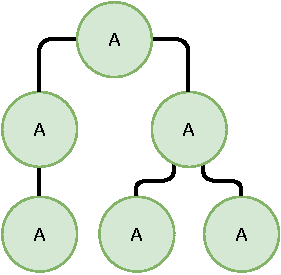
\includegraphics[width=4.5cm]{images/chapter_2/graph_a.pdf}
    \caption{}
    \label{figure:a}
  \end{subfigure}
  \begin{subfigure}[b]{0.3\textwidth}
    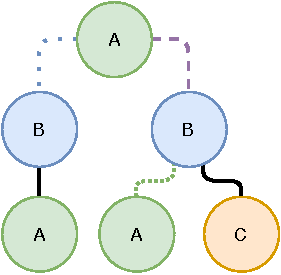
\includegraphics[width=4.5cm]{images/chapter_2/graph_b.pdf}
    \caption{}
    \label{figure:b}
  \end{subfigure}
  \begin{subfigure}[b]{0.3\textwidth}
    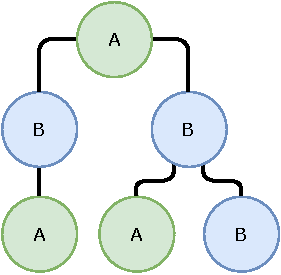
\includegraphics[width=4.5cm]{images/chapter_2/graph_c.pdf}
    \caption{}
    \label{figure:c}
  \end{subfigure}
\fontsize{9}{10.8}\caption[Types of Graphs According to Input]{Three types of graphs, according to the type of input: \textbf{(a)} homogeneous, \textbf{(b)} heterogeneous, and \textbf{(c)} bipartite graph.}
\label{figure:graphs}
\end{figure}

In the last few years, some works have emerged regarding heterogeneous graph attention mechanisms. \cite{zhou2019hahe} proposed a Hierarchical Attentive Heterogeneous information network Embedding (HAHE) model that takes into account personalized preferences of different nodes on different meta paths in each semantic space. Similarly, in the biomedical domain, \cite{hosseini2019hierarchical} introduced a target-aware hierarchical attention mechanism for diagnosis prediction using Electronic Health Records (EHR). Also, \cite{yang2020interpretable} tries to bridge the shortcomings of previous systems, regarding flexibility in exploiting all possible meta-paths and scalability, by proposing an interpretable and efficient Heterogeneous Graph Convolutional Network (ie-HGCN) to learn representations of nodes. 

Using heterogeneous graphs attention mechanisms to represent indirect relations between different type entities, such as genes and diseases in the biomedical domain, can be a viable additional external source of knowledge to preexisting deep learning RE systems \citep{wu2020comprehensive}. Thus, enabling us to find representations of an indirect relation between two entities using knowledge graphs. The candidate knowledge graphs to implement heterogeneous graphs attention mechanisms could be ontologies representing the entities of interest and their semantic relationships in a given domain. \cite{li2020bio} took an attention mechanism approach to identify protein-protein interactions, using attention mechanisms within a Bidirectional Long-Short Term Memory neural network (BiLSTM). Their attention mechanism leads on the knowledge base (KB) information from BioModels\footnote{\url{https://www.ebi.ac.uk/biomodels/}} and filters the information with the weight vector to reflect how external information is relevant to the current state $h_t$ (Section \hyperlink{2.1.4.2}{2.1.4.2}). However, they struggle with KB coverage and how to efficiently integrate external information and do not use heterogeneous graph attention mechanisms, which could be of great value for information retrieval from biomedical literature. 

According to \cite{ehrlinger2016towards}, the difference between a knowledge graph and an ontology could be interpreted either as a matter of quantity (e.g., a large ontology) or of extended requirements (e.g., a built-in reasoner that allows new knowledge to be derived). However, the consensus is that ontologies are smaller collections of hand-curated assertions, usually for solving a domain-specific problem, upping their reliability. 

\subsubsection{Ontologies}

An ontology is a structured way of providing a common vocabulary in which shared knowledge is represented \citep{gruber1993translation}. Word embeddings can learn how to detect relations between entities but manifest difficulties in grasping the semantics of each entity and its specific domain. Domain-specific ontologies provide and formalize this knowledge. Biomedical ontologies are usually structured as a directed acyclic graph, where each node corresponds to an entity, and the edges correspond to known relations between those entities. Thus, a structured representation of the semantics between entities and their relations, an ontology, allows us to use it as an added feature to a machine learning classifier. Some of the biomedical entities structured in publicly available ontologies are genes properties/attributes (Gene Ontology (GO) \citep{ashburner2000gene}), phenotypes (Human Phenotype Ontology (HPO) \citep{robinson2010human}), diseases (Human Disease Ontology (DO) \citep{schriml2012disease}), and chemicals (Chemical Entities of Biological Interest (ChEBI) \citep{hastings2016chebi}). All of these entities participate in relations with different and same domain-type entities. Hence, the information about each entity on a semantic level adds a new layer of knowledge to increase the performance of RE classifiers. 

Non-biomedical models using ontologies as an added source of information to neural networks are becoming widespread for several tasks. \cite{li2016learning} propose using word sense definitions provided by the WordNet ontology to learn one embedding per word sense for word sense disambiguation tasks. \cite{ma2017ontology} focus their work on semantic relations between ontologies and documents, using the DBpedia ontology. Some researchers explored graph embedding techniques \citep{goyal2018graph} that convert relations to a low dimensional space which represents the structure and properties of the graph. Other researchers have combined different sources of information, including ontological information, to do multi-label classification \citep{kong2013multi} and used ontology concepts to represent word tokens \citep{dasigi2017ontology}.

However, few authors have used biomedical ontologies to perform RE. Textpresso \citep{muller2004textpresso} is a text-mining system that works as a search engine for individual sentences acquired from the full text of scientific articles and articles. It integrates biomedical ontological information (e.g., of genes, phenotypes, and proteins), allowing for article and sentence search a query by term. The integration of ontological information allows for semantic queries. This system helps database curation by automatically extracting biomedical relations. The IICE \citep{lamurias2014identifying} system uses kernel-based support vector machines and an ensemble classifier to identify and classify drug-drug interactions, linking each chemical compound to the ChEBI ontology. \cite{tripodi2017knowledge} system focuses on drug-gene/protein interaction discovery to aid database curation using ChEBI and GO ontologies. BO-LSTM \citep{lamurias2019bo} incorporates ancestry information from biomedical ontologies with deep learning to extract relations from the text, such as drug-drug interactions and gene-phenotype relations. 

\section{Evaluation for Relation Extraction}

The evaluation of deep learning systems is done by applying the trained models to a test set. Gold standard test sets are manually curated or annotated by domain experts and unseen by the system. For a binary sentence-based RE task, the test set should correspond to the list of pairs of entities (e.g., person-organization or gene-disease pairs) that co-occur in the same sentences and their relation.

\subsection{Results}

For any given information extraction system, it is necessary to define what constitutes a positive and negative result, particularly in the biomedical domain. Researchers and clinicians need to have access not only to known relations between biomedical entities but also to relations that were already disproven. Accessible negative results limit their search space and prevent the costly re-exploration of research hypotheses. However, most biomedical RE datasets do not seek to distinguish between a false and a negative relation between two biomedical entities, and few knowledge bases hold negative examples. Some domain-specific exceptions are worth noticing, such as the Negatome database \citep{blohm2014negatome} for protein-protein interactions and the phenotype-disease relations annotation file made available by the Human Phenotype Ontology (HPO) organization \citep{robinson2010human} that contains both positive and negative relations.

A false relation should express a context where the entities are not related. In contrast, a negative relation should explicitly express a context where there is an affirmation of no association between the two entities. Furthermore, datasets created using distant supervision techniques also have some false negative relations that constitute undocumented/unknown relations \citep{sousa2019silver}. These relations are not marked true because they are not described in a knowledge base at the moment of the dataset creation, even though upon reading the context of these relations within their respective sentences, one can support a true relation. Unknown relations are good examples of hypotheses to be further explored by researchers and clinicians and can be of use to effectively populate the biomedical relations knowledge bases. In RE tasks, the binary type of results possible are Relation that can be either positive or negative, and No Relation that is only false, shown in Table \ref{table:evaluation}.

\begin{table}[ht]
\centering
\caption[Types of Results Obtained with an Information Extraction System for a Relation Extraction Task]{Types of results obtained with an information extraction system for a RE task}
\begin{tabular}{ccc}
\hline
Annotator (Gold Standard) & System & Classification\\
\hline
\multirow{2}{*}{Relation} & Relation & True Positive (TP) \\
 & No Relation & False Negative (FN) \\ 
\hline
\multirow{2}{*}{No Relation} & Relation & False Positive (FP) \\
 & No Relation & True Negative (TN) \\
 \hline
\end{tabular}
\label{table:evaluation}
\end{table}

\subsection{Metrics}

The primary goal of a given information retrieval system is to maximize the number of TP and TN. To compare results obtained with different datasets or different tools, we have three distinct evaluation metrics: recall, precision, and F-measure. Precision represents how often the results are correct, recall the number of correct results identified, and F-measure is a combination of both metrics to express overall performance, being the harmonic mean of precision and recall:

\begin{equation}
F-measure = \frac{2\times Precision\times Recall}{Precision + Recall} = \frac{2 TP}{2 TP + FP + FN}
\label{equation:evaluation}
\end{equation} 

Occasionally, Accuracy is also used to consider the number of TNs and expresses the overall correctness of a classification model. It represents the proportion of correctly classified instances (or predictions) of a dataset's total number of instances.

Some approaches also consider the Area under the precision-recall curve (AUPRC) to measure the trade-off between precision and recall at various thresholds. It comprehensively evaluates a model's performance across different operating points and is particularly useful when dealing with imbalanced datasets. Also, the Area under the receiver operating characteristic curve (AUROC) measures the trade-off between true positive rate (TPR or recall) and false positive rate (FPR) at various classification thresholds. While commonly used in binary classification tasks, it may not be the most suitable metric for biomedical relation extraction due to class imbalance issues.

Additionally, depending on the specific application and requirements, other metrics such as specificity, sensitivity, and the Matthews correlation coefficient (MCC) may be used to evaluate the performance of biomedical relation extraction models. 

Also, it is important to note that statistical significance testing and p-values can be relevant in specific research scenarios in biomedical relation extraction, where they are used to validate the significance of associations or correlations between variables or features. 

\subsection{Datasets}

There are three types of datasets for RE. The first type is the \textbf{traditional information extraction datasets}, where relations are manually annotated and pre-determined. Some examples of these types of biomedical datasets:

\begin{itemize}
    \item \textbf{AImed} \citep{mooney2006subsequence} describes interactions between human proteins (e.g, \textit{sigma(K)} interacts with \textit{cwlH}). It consists of 225 Medline abstracts, of which 200 describe interactions, with around 1000 tagged interactions.
    \item \textbf{BioNLP Shared Task} \citep{kim2011overview} describes relations between proteins and components, and sub-units and complexes (e.g., \textit{fimV} regulates \textit{FimS}). The corpus consists of 1210 Medline abstracts with 2834 relations. 
    \item \textbf{ADE-V2} \citep{gurulingappa2012development} describes relations between drugs and drug-related adverse effects (e.g., \textit{ticlopidine} causes \textit{severe aplastic anemia}). It consists of 2872 PubMed documents describing 7100 relations. 
    \item \textbf{DDI} \citep{herrero2013ddi} describes interactions between pharmacological substances/drugs (e.g., \textit{perindoprilat} effects \textit{diuretics}). The corpus consists of 792 texts selected from the DrugBank database and 233 Medline abstracts and describes 34449 relations. 
    \item \textbf{BC5CDR} \citep{li2016biocreative} describes relations between chemicals and diseases (e.g., \textit{timolol} effects \textit{myocardial infarction}). The corpus consists of 1500 PubMed articles with 3116 chemical-disease interactions.
    \item \textbf{BioRED} \citep{luo2022biored} describes relations pairs between genes/proteins, diseases, and chemicals (e.g., \textit{D374Y} positively correlates to \textit{autosomal dominant hypercholesterolemia}). It consists of 600 PubMed abstracts with 6503 relations. 
\end{itemize}

The second type is \textbf{open information extraction datasets}, where relations are manually annotated but can be of any type \citep{fader2011identifying,del2013clausie,mesquita2013effectiveness}. 

Finally, the third type is \textbf{distantly supervised datasets}, where distant supervision is applied, and the relations are usually pre-determined. This last type has been rapidly expanding for being less costly and time-consuming than the previous \citep{riedel2010modeling}. One example of these datasets in the biomedical domain is the PGR Corpus \citep{sousa2019silver} that describes relations between human phenotypes and genes and precedes the work developed in this thesis.

\section{Current Challenges} 

Biomedical RE has its domain-specific challenges to overcome, such as sentence and entity complexity, lack of models for languages other than English, lack of standardization of nomenclature for biomedical entities such as human phenotypes and diseases, and lack of datasets to train models (in English and other languages). 

To tackle sentence and entity complexity, we have some preprocessing tools that aim to mask the information deemed unnecessary for RE \citep{miwa2010entity,lee2020biobert}. Thus, instead of contemplating the whole region between the target pair, this region is simplified by giving different weights to each element in the sentence or even removing unnecessary words that are not relation-related. The use of word embeddings explicitly trained for the biomedical domain has shown to be effective for all biomedical NLP-related tasks \citep{lee2020biobert,scibert}.

Biomedical RE targeting non-English literature is essential due to the sheer quantity of biomedical research written in other languages (approximately 16\% just in PubMed\footnote{as of January 2022}). For instance, clinical reports are almost always written in the medical practitioner/patient native language \citep{10.1093/database/bax064}. This literature holds relevant information that can be of interest to support or discard a scientific hypothesis \citep{nussbaumer2020excluding}, and it is rarely considered \citep{di2017publish}. Some works target biomedical RE in non-English languages \citep{6103454}. At the same time, other researchers are dedicated to the translation of biomedical resources such as ontologies like the Human Phenotype Ontology to other languages such as Spanish and Portuguese\footnote{\url{https://github.com/drseb/HPO-translations}}. 

The lack of standardization of nomenclature for biomedical entities is prominent since biomedical NLP first emerged \citep{leser2005makes,horwitz2011naming}. Although this problem can seem to be a NER problem, since NER is a necessary precedent step to RE, it also affects RE, particularly with entities that use more than one word. The multi-word entities, such as the disease \textit{breast cancer}, come with some challenges. The first is if we consider more than one level relation by dividing multi-word entities, for instance, \textit{breast cancer} and the gene \textit{BRACA1} and \textit{cancer} and the gene \textit{BRACA1}. The second challenge is if we can imply the two relations even if the KB supporting the gold standard relations only considers the gene \textit{BRACA1} having a relation with \textit{cancer} and not \textit{breast cancer}, for instance. In some examples, it is easy for us to consider relation transfer, but for others, it is more challenging. It is not trivial to formulate a rule that fits all cases for all the different biomedical entities. 

Finally, the fourth challenge for the biomedical RE task is the lack of annotated datasets to train models. One solution can be creating these datasets through distant supervision allied with crowdsourcing, although it still brings some concerns, such as reliability and bias depending on the platform and pre-defined settings.  

The following four chapters tackle the absence of structured, high-quality knowledge integrated into RE systems (Chapters 3, 4, and 5) and the need for gold standard corpora to validate those systems (Chapter 6). Chapter 7 assesses the work done throughout the thesis by applying it to multiple community-driven workshops and challenges, among other applications.  

